\documentclass[
bachelor
, english
, a4paper
, 11pt
, oneside
, webreferences
, glossary
, indextop
, listoflistings
, listofalgorithms
, acronyms
]{INSOthesis}
\inputencoding{utf8}

\thesistitle{
Optimized native implementation of
Lyra2 password hashing scheme in Java
}
\thesisshorttitle{Lyra2 password hashing scheme in Java}
% \thesissubtitle{}
\thesisdate{\today}

% all titles and designations have to be gender-related!
\thesiscurriculum{
Software Engineering and Internet Computing
}{
Software Engineering and Internet Computing
}
\thesisauthor{Aleksandr Lisianoi}
\thesismatrikelno{01527346}

% advisor
%\thesisauthorpreamble {Verfasser}
%\thesisadvisorpreamble {Betreuung}
\thesisadvisorone {Clemens Hlauschek}
\thesisadvisortwo {Clemens Hlauschek}
%\thesisadvisorthree {Vorname Nachname}

% Bibliographie file
\bibliography{bibliography/references}

\hypersetup{
  %colorlinks=false % enable and disable frames around links
}

%%%%%%%%%%%%%%%%%%%%%%%%%%%%%%%%%%%%%%%%%%%%%
%
% Can be used to add additional information
%
%%%%%%%%%%%%%%%%%%%%%%%%%%%%%%%%%%%%%%%%%%%%%
% \AfterTitlePages{}
% \AfterDeclaration{}
% \AfterAcknowledgements{}
% \AfterAbstract{}
% \AfterListOfFigures{}
% \AfterListOfTables{}
% \AfterAbbreviations{}
% \AfterBibliography{}

\renewcommand\afterchapternum{\hspace{1em}}
\begin{document}

\maketitle

%%%%%%%%%%%%%%%%%%%%%%%%%%%%%%%%%%%%%%%%%
%%%   CONTENTS    %%%%%%%%%%%%%%%%%%%%%%%
%%%%%%%%%%%%%%%%%%%%%%%%%%%%%%%%%%%%%%%%%

%%%%%%%%%%%%%%%%%%%%%%%%%%%%%%%%%%%%%%%%%%%%%%%%%%%%%%%%%%%%%%%%%%%%%%%%
\chapter{Introduction}
\label{sec:introduction}
%%%%%%%%%%%%%%%%%%%%%%%%%%%%%%%%%%%%%%%%%%%%%%%%%%%%%%%%%%%%%%%%%%%%%%%%
Passwords are currently the backbone of user authentication. Usually, passwords are stored in a hashed form in some kind of a database. Such databases are fairly often compromised and then the hashing mechanism is what stands between the attacker and the password cleartext.

%=======================================================================
\section{Problem Description}
%=======================================================================
Processing power increases with time while simultaneously getting cheaper. This works both for the legitimate users as well as the attackers. Password Hashing Schemes (PHSs) are therefore continuously adjusted to stay irreversible. However, recent advances in highly parallelized hardware (conventional multicore GPUs as well as the more specialized FPGAs and ASICs) present a new challenge for the commonly used cryptographic hash functions. An attacker can heavily parallelize the computation, trying several thousands of password and salt combination in the time it takes a legitimate user to compute just one.

In order to limit the throutput a potential attacker could achieve, the Password Hashing Competition was announced in 2013 and concluded in 2015 \cite{wetzels:2016:phc}. Its evaluation criteria stress that proposed candidates should provide minimal speed-up for the highly parallelized hardware. The winner was declared to be Argon2 \cite{biryukov:2015:argon2} and special recognition was also given to Catena \cite{forler:2013:catena}, Lyra2 \cite{andrade:2016:lyra2,marcos:2015:lyra2}, Makwa \cite{pornin:2015:makwa} and yescrypt \cite{peslyak:2015:yescrypt}.

%=======================================================================
\section{Motivation}
%=======================================================================
Even though the theoretical designs and their proof-of-concept implementations were presented back in 2015, the adoption of these new cryptographic algorithms could be better. There are many ways to do so: provide better documentation, detailed usage examples and success stories. Porting an existing implementation into another programming language can also result in an adoption boost.

%=======================================================================
\section{Contribution}
%=======================================================================
This work describes the porting process of the Lyra2 reference implementation into Java. The resulting implementation is hosted in the Maven central repository \cite{maven:2017:lyra2} as well as on GitHub \cite{github:2017:lyra2-java}. This makes it available for seamless inclusion as a dependency into any Java project. It is licensed under the MIT license which is a well-known permissive software license. Finally, the source code is publicly available and can be inspected or improved if necessary.

The primary goal of this porting effort is to provide a drop-in replacement for the reference implementation. Given the same input parameters, both implementations should produce the same hash values. Although this might sound like an automatic requirement, it is not in fact the case. The paper will highlight the challenges in details about the Java implementation section \ref{sec:java-implementation}.

The secondary goal is to compare the ported implementation to the original. The comparison project is done in the spirit of reproducible research, is hosted publicly on GitHub \cite{github:2017:lyra2-compare} and can be used to verify the results presented in this paper.

The final goal is to use the ported implementation to write an Android application. Section \ref{sec:mobile-application} demonstrates the ease of deployment of Lyra2 on a platform where using the reference implementation is not as straightforward.

%=======================================================================
\section{Outline of the Work}
%=======================================================================

\emph{Section \ref{sec:fundamentals}} is devoted to theoretical background. It opens with the basic definitions as well as a brief mention of existing password hashing solutions which are either not memory-hard or have other notable drawbacks. A short description of Lyra2 follows in \ref{sec:lyra2-brief-description}, introducing the notion of a sponge function as well as a duplex construction. The main part of that section deals with the memory matrix created by Lyra2 and the way it interacts with the duplex constructions during the different phases of the algorithm.

\emph{Section \ref{sec:implementation-details}} covers implementation details. It begins with a quick discussion of the reference implementation \ref{sec:reference-implementation}. It outlines the build system and the various possible configurations of Lyra2. The section concludes with an extension of the build system which allows to compile several configurations at once as well as compute a bulk of hash values. The ported Lyra2 project is discussed next in \ref{sec:java-implementation}. It first deals with the transition from a function-based to an object-oriented project. The most important classes are shown on an UML diagram \ref{fig:uml}. Several classes exist to circumvent specific porting challenges. These challenges are explained and illustrated. In particular, the endianness issue is shown in figure \ref{fig:little-endian} and a rotation trick for the Blake2b-based sponge is shown in figure \ref{fig:sponge-blake2b}.

\emph{Section \ref{sec:results}} summarizes the results. It begins with the demonstration that both projects produce the same hash values given the same inputs \ref{sec:it-works}. First, a manual testing session is recorded in \ref{sec:manual-testing}. A section on continuous integration follows in \ref{sec:automated-testing}. Then the performance comparison is presented in section \ref{sec:performance-comparison}. Due to a large number of configurable parameters in Lyra2, the first comparisons fix time- and memory costs (respectively, subsections \ref{sec:fixed-time-cost} and \ref{sec:fixed-memory-cost}). Section \ref{sec:no-fixed-costs} then deals with both changing time- and memory costs, resulting in several thousands of measurements displayed. A comparison conclusion is made in \ref{sec:comparison-conclusion}. Finally, an Android mobile application is presented in \ref{sec:mobile-application}.

%%%%%%%%%%%%%%%%%%%%%%%%%%%%%%%%%%%%%%%%%%%%%%%%%%%%%%%%%%%%%%%%%%%%%%%%
\chapter{Theoretical Background}
\label{sec:fundamentals}
%%%%%%%%%%%%%%%%%%%%%%%%%%%%%%%%%%%%%%%%%%%%%%%%%%%%%%%%%%%%%%%%%%%%%%%%

A \emph{sponge function} or a \emph{sponge construction} is a class of algorithms with finite internal state that take an input bit stream of any length and produce an output bit stream of any desired length \cite{wiki:2017:sponge-function}. The internal state \(S\) consists of \(w = b + c\) bits, where \(w\) is known as the \emph{width} of the sponge, \(b\) is called its \emph{bitrate} and \(c\) its \emph{capacity}. At the heart of every sponge function lies a \emph{fixed-width permutation} \(f\) which takes \(w\) bits as input and produces \(w\) bits as output. A common example of \(f\) is Blake2b, which in its 64-bit modification operates on 128-byte chunks.

As shown in figure \ref{figure:sponge-construction}, a sponge function conceptually consists of two parts: the absorbing and the squeezing phase. To start with, an incoming message is padded so that its length is a multiple of \(b\) bits. Secondly, the internal state of the sponge is initialized with zeros. Then the absorbing phase begins: the next \(b\) bits of the message are XOR-ed with the first \(b\) bits of \(S\) and then the \(f\) permutation is applied to the whole \(S\). This process repeats until the entire message has been absorbed. At this point the squeezing phase starts: the first \(b\) bits of \(S\) are emitted and then the \(f\) permutation is applied to the whole \(S\). This keeps going until the desired output length is reached.

\begin{figure}
  \begin{tikzpicture}[
  ostyle/.style={
      shape=rectangle
      ,draw
      ,minimum width=0.5cm,
    }
    ,fstyle/.style={
      shape=rectangle
      ,draw
      ,rounded corners=5pt
      ,minimum width=0.5cm
      ,minimum height=5cm
      }
    ,xstyle/.style={
    }
  ]

  \coordinate (A0) at (-0.5, 5) {};
  \coordinate (A1) at (-0.5, 3) {};
  \coordinate (A2) at (-0.5, 0) {};

  \draw [<->,semithick] (A0) to node [left] {\(b\)} (A1);
  \draw [<->,semithick] (A1) to node [left] {\(c\)} (A2);

  \node [ostyle,minimum height=2cm] (00) at (0.5, 4  ) {\(0\)};
  \node [ostyle,minimum height=3cm] (01) at (0.5, 1.5) {\(0\)};

  \node [shape=rectangle,draw] (padded message) at (-0.5, 6) {padded message};

  \coordinate (y0) at (1.5, 6) {};
  \coordinate (y1) at (3.5, 6) {};
  \coordinate (y2) at (5.5, 6) {};
  \coordinate (y3) at (7.5, 6) {};
  \coordinate (y4) at (9.5, 6) {};
  \draw [-] (padded message) to (y0) to (y1) to (y2);

  \node [xstyle] (x0) at (1.5, 4) {\(\oplus\)};
  \node [xstyle] (x1) at (3.5, 4) {\(\oplus\)};
  \node [xstyle] (x2) at (5.5, 4) {\(\oplus\)};
  \coordinate (x3) at (7.5, 4) {};
  \coordinate (x4) at (9.5, 4) {};

  \node [shape=rectangle] (absorb) at (3.5, -1) {absorbing phase};
  \node [shape=rectangle] (squeeze) at (9.5, -1) {squeezing phase};

  \draw [thick,dashed] (7.25, 6.5) -- (7.25, -1.5);

  \draw [->] (y0) to node [right,near start] {1\textsuperscript{st} \(b\) bits} (x0);
  \draw [->] (y1) to node [right,near start] {2\textsuperscript{nd} \(b\) bits} (x1);
  \draw [->] (y2) to node [right,near start] {3\textsuperscript{rd} \(b\) bits} (x2);
  \draw [->] (x3) to node [right,near end] {1\textsuperscript{st} \(b\) bits} (y3);
  \draw [->] (x4) to node [right,near end] {2\textsuperscript{nd} \(b\) bits} (y4);

  \node [fstyle] (f0) at ( 2.5, 2.5) {\(f\)};
  \node [fstyle] (f1) at ( 4.5, 2.5) {\(f\)};
  \node [fstyle] (f2) at ( 6.5, 2.5) {\(f\)};
  \node [fstyle] (f3) at ( 8.5, 2.5) {\(f\)};
  \node [fstyle] (f4) at (10.5, 2.5) {\(f\)};

  \draw [->] (00) to (x0);
  \draw [->] (x0) -- (x0 -| f0.west);
  \draw [->] ($(f0.east) + (0, 1.5)$) -- (x1);
  \draw [->] (x1) -- (x1 -| f1.west);
  \draw [->] ($(f1.east) + (0, 1.5)$) -- (x2);
  \draw [->] (x2) -- (x2 -| f2.west);
  \draw [-] ($(f2.east) + (0, 1.5)$) -- (x3);
  \draw [-] (x3) -- ($(f3.west) + (0, 1.5)$);
  \draw [-] ($(f3.east) + (0, 1.5)$) -- (x4);
  \draw [-] (x4) -- ($(f4.west) + (0, 1.5)$);
  \draw [->] ($(f4.east) + (0, 1.5)$) -- ($(f4.east) + (1, 1.5)$);

  \draw [->] (01) -- (01 -| f0.west);
  \draw [->] ($(f0.east) + (0, -1)$) -- ($(f1.west) + (0, -1)$);
  \draw [->] ($(f1.east) + (0, -1)$) -- ($(f2.west) + (0, -1)$);
  \draw [->] ($(f2.east) + (0, -1)$) -- ($(f3.west) + (0, -1)$);
  \draw [->] ($(f3.east) + (0, -1)$) -- ($(f4.west) + (0, -1)$);
  \draw [->] ($(f4.east) + (0, -1)$) -- ($(f4.east) + (1, -1)$);

  \end{tikzpicture}
  \caption{The Sponge Construction}
  \label{figure:sponge-construction}
\end{figure}

\begin{figure}
  \begin{tikzpicture}[
  ostyle/.style={
      shape=rectangle
      ,draw
      ,minimum width=0.5cm,
    }
    ,fstyle/.style={
      shape=rectangle
      ,draw
      ,rounded corners=5pt
      ,minimum width=0.5cm
      ,minimum height=5cm
      }
    ,xstyle/.style={
    }
  ]

  \coordinate (A0) at (-0.5, 5) {};
  \coordinate (A1) at (-0.5, 3) {};
  \coordinate (A2) at (-0.5, 0) {};

  \draw [<->,semithick] (A0) to node [left] {\(b\)} (A1);
  \draw [<->,semithick] (A1) to node [left] {\(c\)} (A2);

  \node [ostyle,minimum height=2cm] (00) at (0.5, 4  ) {\(0\)};
  \node [ostyle,minimum height=3cm] (01) at (0.5, 1.5) {\(0\)};

  \coordinate (x00) at ( 1.5, 6) {};
  \coordinate (x01) at ( 4.5, 6) {};
  \coordinate (x02) at ( 7.5, 6) {};
  \coordinate (x03) at (10.5, 6) {};

  \node [xstyle] (x10) at ( 1.5, 4) {\(\oplus\)};
  \node [xstyle] (x11) at ( 4.5, 4) {\(\oplus\)};
  \node [xstyle] (x12) at ( 7.5, 4) {\(\oplus\)};
  \node [xstyle] (x13) at (10.5, 4) {\(\oplus\)};

  \draw [->] (x00) to node [anchor=south,rotate=90] {1\textsuperscript{st} \(b\) bits} (x10);
  \draw [->] (x01) to node [anchor=south,rotate=90] {2\textsuperscript{nd} \(b\) bits} (x11);
  \draw [->] (x02) to node [anchor=south,rotate=90] {3\textsuperscript{rd} \(b\) bits} (x12);
  \draw [->] (x03) to node [anchor=south,rotate=90] {4\textsuperscript{th} \(b\) bits} (x13);

  \coordinate (x14) at (13.5, 4) {};
  \coordinate (x24) at (13.5, 1.5) {};

  \coordinate (y00) at (3.5, 6) {};
  \coordinate (y01) at (6.5, 6) {};
  \coordinate (y02) at (9.5, 6) {};

  \coordinate (y10) at (3.5, 4) {};
  \coordinate (y11) at (6.5, 4) {};
  \coordinate (y12) at (9.5, 4) {};

  \draw [<-] (y00) to node [anchor=south,rotate=90] {1\textsuperscript{st} \(b\) bits} (y10);
  \draw [<-] (y01) to node [anchor=south,rotate=90] {2\textsuperscript{nd} \(b\) bits} (y11);
  \draw [<-] (y02) to node [anchor=south,rotate=90] {3\textsuperscript{rd} \(b\) bits} (y12);

  \draw [->] (y10) -- (y00);
  \draw [->] (y11) -- (y01);
  \draw [->] (y12) -- (y02);

  \node [fstyle] (f0) at ( 2.5, 2.5) {\(f\)};
  \node [fstyle] (f1) at ( 5.5, 2.5) {\(f\)};
  \node [fstyle] (f2) at ( 8.5, 2.5) {\(f\)};
  \node [fstyle,dashed] (f3) at (11.5, 2.5) {\(f\)};

  \draw [->] (00) to (x10);
  \draw [->] (x0) -- (x0 -| f0.west);
  \draw [->] ($(f0.east) + (0, 1.5)$) -- (x11);
  \draw [->] (y10) -- (y00);
  \draw [->] (x11) -- (x11 -| f1.west);
  \draw [->] ($(f1.east) + (0, 1.5)$) -- (x12);
  \draw [->] (x12) -- (x12 -| f2.west);
  \draw [->] ($(f2.east) + (0, 1.5)$) -- (x13);
  \draw [->] (x13) -- ($(f3.west) + (0, 1.5)$);
  \draw [->,dashed] ($(f3.east) + (0, 1.5)$) -- (x14);
  % \draw [-] ($(f3.east) + (0, 1.5)$) -- (x4);
  % \draw [-] (x4) -- ($(f4.west) + (0, 1.5)$);
  % \draw [->] ($(f4.east) + (0, 1.5)$) -- ($(f4.east) + (1, 1.5)$);

  \draw [->] (01) -- (01 -| f0.west);
  \draw [->] ($(f0.east) + (0, -1)$) -- ($(f1.west) + (0, -1)$);
  \draw [->] ($(f1.east) + (0, -1)$) -- ($(f2.west) + (0, -1)$);
  \draw [->] ($(f2.east) + (0, -1)$) -- ($(f3.west) + (0, -1)$);
  \draw [->,dashed] ($(f3.east) + (0, -1)$) -- (x24);
  % \draw [->] ($(f3.east) + (0, -1)$) -- ($(f4.west) + (0, -1)$);
  % \draw [->] ($(f4.east) + (0, -1)$) -- ($(f4.east) + (1, -1)$);

  \end{tikzpicture}
  \caption{The Duplex Construction}
  \label{figure:duplex-construction}
\end{figure}

%=======================================================================
\section{State of the Art}
%=======================================================================

%%%%%%%%%%%%%%%%%%%%%%%%%%%%%%%%%%%%%%%%%%%%%%%%%%%%%%%%%%%%%%%%%%%%%%%%
\chapter{Konkrete Problemstellung -- Umfeldbeschreibung}
\label{sec:problemdescription}
%%%%%%%%%%%%%%%%%%%%%%%%%%%%%%%%%%%%%%%%%%%%%%%%%%%%%%%%%%%%%%%%%%%%%%%%

In diesem Kapitel wird die eigentliche Problemlösung in einem oder mehreren Unterkapiteln ausgeführt. Die Strukturierung dieser Kapitel ist naturgemäß sehr stark von der konkreten Aufgabenstellung abhängig. Der Name dieses Kapitels ist anzupassen, z.B. Umfeldbeschreibung -- Fallbeispiel \dots, konkreter schreiben je nach Art Diplomarbeit/Fragestellung.
\makeatletter\ifthesis@masterthesis
Nachfolgend einige Beispiele für unterschiedliche Arten von Diplomarbeiten.

Bei einer Software-Entwicklungsarbeit bieten sich folgende Unterkapitel an:
\begin{itemize}
	\item Im Kapitel \enquote{Design} sollte die konzeptionelle Lösung vorgestellt, diskutiert und begründet werden. Das Ergebnis dieses Kapitels könnte beispielsweise eine Protokoll-Architektur sein.
	\item Im Kapitel \enquote{Modelle} erfolgt üblicherweise das Feindesign. In diesem Kapitel könnten beispielsweise einzelne Protokolle bzw. Algorithmen aus der vorher definierten Protokoll-Architektur eingeführt und diskutiert werden. Achtung: Generell darauf achten, bei der eingangs erläuterten Notation zu bleiben und nicht Synonyme zu verwenden, verwirrt den Leser.
	\item Das Kapitel \enquote{Implementierung} sollte sich dann vorwiegend mit den Details der Umsetzung befassen. In diesem Kapitel sollte nur im Ausnahmefall exemplarisch Quellcode vorgesehen werden. Vielmehr sollten alle Probleme, die bei der Realisierung aufgetreten sind, dokumentiert, interpretiert und die Lösung erläutert werden.
\end{itemize}

Bei einer Arbeit zu einem abstrakteren Thema, bei dem ein oder mehrere Fallbeispiele aus der industriellen Praxis bearbeitet werden, bieten sich folgende Unterkapitel an:
\begin{itemize}
	\item Im Unterkapitel \enquote{Analyse der Problemstellung} wird die konkrete Problemstellung (die Situation im betrachteten Unternehmen) der Fallbeispiele beschrieben. Das Ergebnis dieses Kapitels könnte eine schematische Netzwerk- oder Applikationsarchitektur sein.
	\item Im Unterkapitel \enquote{Fallbeispiel} sollte sich (analog zur Implementierung in der Software-Entwicklung) mit den konkreten Details der Umsetzung befassen. Hier wird dargelegt, wie das zuvor identifizierte Lösungsschema konkret zur Anwendung gelangen kann bzw. welche Probleme während des Umsetzungsprojekts aufgetreten sind.
\end{itemize}

Bei einer Arbeit, deren Grundlage eine Auswahl eines Softwaresystems ist, bieten sich folgende Unterkapitel an:
\begin{itemize}
	\item IST-Analyse
	\item Hardware und Softwareausstattung
	\item Beschreibung der Geschäftsprozesse
	\item Schwachstellenanalyse des Unternehmens
	\item SOLL-Konzeption
	\item Auswahlverfahren möglicher verfügbarer Systeme -- Kriterienkatalog
	\item Einführung des neuen Systems
\end{itemize}

Bei einer Arbeit, deren Fokus auf der Durchführung und Auswertung von Fragebögen liegt, bieten sich folgende Unterkapitel an:
\begin{itemize}
	\item Im Kapitel \enquote{Problemstellung und Fragebogendesign} wird die fachliche Problemstellung detailliert erläutert und der Inhalt des Fragebogens in Bezug zur Problemstellung dargestellt.
	\item Im Kapitel \enquote{Befragungsmethode} werden die Untersuchungsobjekte (z.B. Praktische Ärzte), die Grundgesamtheit (Anzahl praktische Ärzte in Venezuela), Stichprobengesamtheit und das Verfahren zur Stichprobenziehung und das Erhebungsverfahren (Verteilung und Rücklauf der Fragebögen) beschrieben.
	\item Im Kapitel \enquote{Auswertungsmethode} werden die möglichen Auswertungsmethoden aufgelistet und ggf. begründet die ausgewählte Methode beschrieben.
	\item Im Kapitel \enquote{Befragungsdurchführung} wird die Untersuchungsdurchführung (z.B. Zeit, Ort der Befragung, Zeitraum der gesamten Befragung, besondere für das Untersuchungsergebnis oder zukünftige Forschungsarbeiten relevante Vorkommnisse etc.) dargestellt.
\end{itemize}

Hier intensive Rücksprache mit Ihren jeweiligen Fachbetreuern halten, mehrere Diplomarbeiten der Fakultät zu diesem Themenbereich durchsehen. Unabhängig vom Typ der Diplomarbeit werden im nachfolgenden Kapitel die konkreten Ergebnisse beschrieben.
\fi\makeatother
\chapter{Hinweise zur Literatur}
\label{sec:references}

\section{Literatursuche}

Der Vollzugang zu einigen Publikationen ist nur intern aus dem TU-Netz möglich. Um auf möglichst viele Papers extern zugreifen zu können, wird von der TU Wien eine \href{http://www.zid.tuwien.ac.at/tunet/vpn/extern/}{VPN-Zugangsmöglichkeit} angeboten, diesen VPN-Zugang bitte gleich einrichten.

Besonders ergiebig sind folgende Search-Engines:\\
\href{http://academic.research.microsoft.com/}{Microsoft Academic}\\
\href{http://dl.acm.org/}{ACM-Datenbank}\\
\href{http://scholar.google.com/}{Google Scholar}

Wir empfehlen, vor Beginn Ihrer Arbeit einige Diplomarbeiten, die am INSO oder generell an der Fakultät für Informatik verfaßt wurden, zu Ihrem Themenbereich zu suchen und Aufbau, Schreibstil, Art der Abbildungen etc. durchzuschauen. Arbeiten finden Sie \href{http://media.obvsg.at/tuw?query=grechenig&metaname=swishdefault&submit=Suche+starten&sbm=tuw*&lbm=*&lbc=*&searchtype=sim&.cgifields=metaname}{hier}.

Weitere Datenbanken und Suchmaschinen:\\
\href{http://rzblx1.uni-regensburg.de/ezeit/search.phtml?bibid=UBTUW&colors=7&lang=de}{Elektronische Zeitschriftenbibliothek der TU Wien}\\
\href{http://citeseer.ist.psu.edu/index;jsessionid=BF9BD5A89D42210F60E5CA88B40BAD9C}{Scientific Literature Digital Library (CiteSeer)}\\
\href{http://www.ingentaconnect.com/}{Ingenta}\\
\href{http://www.theiet.org/resources/inspec/}{INSPEC}

Journals:\\
\href{http://ieeexplore.ieee.org/}{IEEE - Institute of Electrical and Electronics Engineers, Inc. - Library}\\
\href{http://www.springerlink.com/?MUD=MP}{Verlag Springer - Springer Link}\\
\href{http://www.elsevier.com/wps/find/homepage.cws_home}{Elsevier}

Bibliotheken und Online-Kataloge:\\
\href{http://search.obvsg.at/primo_library/libweb/action/search.do?vid=ACC}{Online-Kataloge des Österreichischen Bibliothekenverbundes}\\
\href{http://aleph.ub.tuwien.ac.at/}{Online-Katalog der TU Wien} (ALEPH)\\
\href{http://www.informatik.uni-trier.de/}{Digital Bibliography \& Library Project (DBLP) of University of Trier}\\
\href{http://liinwww.ira.uka.de/bibliography/}{The Collection of Computer Science Bibliographies}

\section{BibLatex}

Biblatex bietet verschiedene Möglichkeiten an, um Literatur zu referenzieren. Die beiden häufigsten Befehle sind \verb|\cite| und \verb|\citeauthor|.

Beispiele wie referenziert werden kann:\\
\citeauthor{fankhauser:2009:softwaretechnik-security} beschreiben in \cite{fankhauser:2009:softwaretechnik-security} \dots\\
In \cite{schanes:2011:voip-fuzzer} zeigen \citeauthor{schanes:2011:voip-fuzzer} wie \dots
Weitere Informationen können in \cite{oasis:2010:homepage} von \citeauthor{oasis:2010:homepage} entnommen werden.

Wir empfehlen JabRef, um die Literaturdatenbank zu verwalten.

\chapter{Algorithmen und Quellcode}

\section{Beispiele für Quellcode}

Beispiel eines Quellcodes ist im Quellcode \ref{lst:shortcode} zu finden.

\begin{lstlisting}[caption={Short code},label=lst:shortcode]
//Start Program
System.out.println("Hello World!");
//End Program
\end{lstlisting}


\section{Beispiele für Algorithmen}

Algorithmus \ref{alg:samplealgorithm} dient als Beispiel.

\begin{algorithm}[t]
\SetKwData{Left}{left}
\SetKwData{This}{this}
\SetKwData{Up}{up}
\SetKwFunction{Union}{Union}
\SetKwFunction{FindCompress}{FindCompress}
\SetKwInOut{Input}{input}
\SetKwInOut{Output}{output}

\Input{A bitmap $Im$ of size $w\times l$}
\Output{A partition of the bitmap}

\BlankLine

\emph{special treatment of the first line}\;
\For{$i\leftarrow 2$ \KwTo $l$}{
\emph{special treatment of the first element of line $i$}\;
\For{$j\leftarrow 2$ \KwTo $w$}{\label{forins}
\Left$\leftarrow$ \FindCompress{$Im[i,j-1]$}\;
\Up$\leftarrow$ \FindCompress{$Im[i-1,]$}\;
\This$\leftarrow$ \FindCompress{$Im[i,j]$}\;
\If(\tcp*[r]{O(\Left,\This)==1}){\Left compatible with \This}{\label{lt}
\lIf{\Left $<$ \This}{\Union{\Left,\This}}\;
\lElse{\Union{\This,\Left}\;}
}
\If(\tcp*[r]{O(\Up,\This)==1}){\Up compatible with \This}{\label{ut}
\lIf{\Up $<$ \This}{\Union{\Up,\This}}\;
\tcp{\This is put under \Up to keep tree as flat as possible}\label{cmt}
\lElse{\Union{\This,\Up}}\tcp*[r]{\This linked to \Up}\label{lelse}
}
}
\lForEach{element $e$ of the line $i$}{\FindCompress{p}}
}
\caption{Sample algorithm}\label{alg:samplealgorithm}
\end{algorithm}

%%%%%%%%%%%%%%%%%%%%%%%%%%%%%%%%%%%%%%%%%%%%%%%%%%%%%%%%%%%%%%%%%%%%%%%%
\chapter{Results}
\label{sec:results}
%%%%%%%%%%%%%%%%%%%%%%%%%%%%%%%%%%%%%%%%%%%%%%%%%%%%%%%%%%%%%%%%%%%%%%%%

This chapter presents the main results of the porting effort. In particular, section \ref{sec:it-works} covers algorithm-level compatibility. Section \ref{sec:performance-comparison} compares performance of the reference and the ported implementations on a number of different configurations of the Lyra2 algorithm. Finally, section \ref{sec:mobile-application} demonstrates the ease of integration of the ported project into an Android mobile application.

\section{Algorithm-level Compatibility}
\label{sec:it-works}

The primary goal of this work was to port Lyra2 to Java so that it would produce the same hash values as the reference implementation when given the same inputs. Such algorithm-level compatibility was achieved and will be demonstrated in section \ref{sec:manual-testing} and section \ref{sec:automated-testing}. The former deals with hand-picked test vectors while the latter demonstrates a reasonably large collection of randomly picked test vectors and a unit-testing framework which uses them to verify hash results.

\subsection{Configuration Choice}
By design Lyra2 has a large number of configurable parameters. This section will provide the reasoning behind the choice of particular values. The short summary can be found in table \ref{table:configuration-summary}.

There are three sponges that could be tested: Blake2b, BlaMka and half-round BlaMka. Only the first two are in the manual testing shortlist because half-round BlaMka is similar to BlaMka. The sponge block size can be either 8, 10 or 12, so the extreme values made it into the shortlist. The columns of the memory matrix can be any positive number. The \path{Lyra2/src/runBenchCPU.sh} benchmarking script as well as other sources suggest that the values of 256 and 512 should be chosen.

Finally, time and memory costs are fixed at an arbitrary value of 100. The output length is chosen to be 10 so that the resulting hash value would fit easily on the page.

\begin{table}
\begin{center}
\begin{tabular}{l r}
Parameter & Value \\ \hline
Sponge & Blake2b, BlaMka \\
Sponge blocks & 8, 12 \\
Sponge rounds & 12 \\
Columns in the memory matrix & 256, 512 \\
Time cost (number of iterations) & 100 \\
Memory cost (number of rows in the memory matrix) & 100 \\
Output length (bytes) & 10 \\
\end{tabular}
\end{center}
\caption{Summary of parameter values for manually tested configurations}
\label{table:configuration-summary}
\end{table}

\subsection{Manual Testing}
\label{sec:manual-testing}

Figure \ref{fig:manual-testing} shows a log of manual tests. New line delimits different Lyra2 configurations. The first line of each group represents a particular configuration group: \verb|--outlen| is the output length, \verb|--tcost| is the time cost, \verb|--mcost| is the memory cost. The second and the forth line in each group is the password and salt pair, and the third and fifth lines are the resulting hash values.

\begin{figure}[p]
\begin{minted}[fontsize=\footnotesize]{shell}
$ lyra2 --sponge blake2b --blocks 8 --columns 256 --outlen 10 --tcost 100 --mcost 100
> "password" "salt"
> 19 FD 3B 50 9A 03 0C DF 95 DA
> "The quick brown fox jumped over the lazy dog" "0123456789"
> 04 A0 BF 30 D1 E5 A5 05 53 E9

$ lyra2 --sponge blake2b --blocks 8 --columns 512 --outlen 10 --tcost 100 --mcost 100
> "password" "salt"
> 73 39 79 B6 C1 3C C1 F3 D7 17
> "The quick brown fox jumped over the lazy dog" "0123456789"
> A1 B0 18 F6 B6 79 5F E0 2A A4

$ lyra2 --sponge blake2b --blocks 12 --columns 256 --outlen 10 --tcost 100 --mcost 100
> "password" "salt"
> 9C 52 2A B9 18 30 F9 E7 09 55
> "The quick brown fox jumped over the lazy dog" "0123456789"
> 7D B2 9D C8 31 B4 E9 0E 10 22

$ lyra2 --sponge blake2b --blocks 12 --columns 512 --outlen 10 --tcost 100 --mcost 100
> "password" "salt"
> AC F2 B6 50 2D BC F0 62 DD 29
> "The quick brown fox jumped over the lazy dog" "0123456789"
> 4F 1B 03 6B C9 A2 09 C4 BC DA

$ lyra2 --sponge blamka --blocks 8 --columns 256 --outlen 10 --tcost 100 --mcost 100
> "password" "salt"
> 53 32 F3 D7 C4 9C 46 38 3C 1B
> "The quick brown fox jumped over the lazy dog" "0123456789"
> E7 6E 4B A0 81 B8 3C CF D6 64

$ lyra2 --sponge blamka --blocks 8 --columns 512 --outlen 10 --tcost 100 --mcost 100
> "password" "salt"
> D9 F9 F5 65 0D 05 88 D0 DF F6
> "The quick brown fox jumped over the lazy dog" "0123456789"
> 3A 3D 40 00 3E 33 44 45 B3 DD

$ lyra2 --sponge blamka --blocks 12 --columns 256 --outlen 10 --tcost 100 --mcost 100
> "password" "salt"
> C1 BC 48 80 99 1C E7 E6 52 18
> "The quick brown fox jumped over the lazy dog" "0123456789"
> 2E 4E 56 C7 5B 3D B7 F9 E0 30

$ lyra2 --sponge blamka --blocks 12 --columns 512 --outlen 10 --tcost 100 --mcost 100
> "password" "salt"
> 82 AF EB 03 5B E7 12 11 BE 63
> "The quick brown fox jumped over the lazy dog" "0123456789"
> F7 A8 56 D5 81 16 AA E5 C7 4D
\end{minted}
\caption{Manual testing protocol, each configuration starts with \texttt{\$}, each password and salt pair is followed by the resulting hash value. The hash value is printed in hexadecimal.}
\label{fig:manual-testing}
\end{figure}

\subsection{Automated Testing}
\label{sec:automated-testing}

The automated testing is possible because of the additional code that was added to the reference implementation. As mentioned in section \ref{sec:reference-implementation}, there is a \verb|harness| branch which could be found in the forked GitHub project \cite{github:2017:lyra-copy} and the corresponding pull request \cite{github:2017:lyra-pr}. This branch introduces the \verb|Lyra2/tests/harness.py| script written in Python 3 which allows to compile several configurations of Lyra2 and then use those to compute and store hash values.

Additionally, the \verb|Lyra2/tests/take.py| Python 3 script was used to choose a number of random hash values from those previously precomputed. These were then used in the Java project to unit-test the implementation. Some of the hash values were also included into the continuous integration service and their status can be verified by visiting \cite{travis:2017:lyra}. However, continuous integration runs only a subset of the vectors that were run locally due to the limited amount of memory available on the remote machines. In conclusion, both manual and automated testing indicate that the ported implementation does not contain immediately visible problems.

\section{Performance Comparison}
\label{sec:performance-comparison}

The single-threaded configuration of the reference C implementation was compared to its ported Java counterpart. For that, a separate GitHub repository was set up in \cite{github:2017:lyra2-compare}. This repository needs to control software written in both C and Java which is why an expressive, high-level scripting language was chosen to complete this task: Python 3.

\subsection{Project Structure}

The comparison project \cite{github:2017:lyra2-compare} is a combination of two Jupyter Notebooks \cite{jupyter:2017:jupyter} and an SQlite database. The two created notebooks follow the producer-consumer strategy. The \mintinline{shell}{src/compare.ipynb} is the producer notebook which is responsible for compiling both C and Java implementations as well as dispatching computation tasks. The results are then collected into the \mintinline{shell}{measurements.db} SQLite database (which also serves as a cache layer). The consumer is the \mintinline{shell}{src/plot.ipynb} notebook which reads the data from the SQLite database and plots the figures shown below.

Lyra2 provides two main adjustable parameters: time and memory cost. Changing both of the parameters at the same time cannot be easily shown on a single graph which is why the comparison contains three main parts. Subsections \ref{sec:fixed-time-cost} and \ref{sec:fixed-memory-cost} show how several Lyra2 configurations behave when time cost and memory cost is fixed, respectively. Subsection \ref{sec:no-fixed-costs} shows a grid of values for both time and memory costs. In all the sections, the two projects are compared using four configurations:

\begin{itemize}
    \item Blake2b sponge with 256 columns, figures \ref{figure:mcost_256}, \ref{figure:tcost_256} and \ref{figure:tcost_mcost_blake2b_256}
    \item Blake2b sponge with 2048 columns, figures \ref{figure:mcost_2048}, \ref{figure:tcost_2048} and \ref{figure:tcost_mcost_blake2b_2048}
    \item BlaMka sponge with 256 columns, figures \ref{figure:mcost_256}, \ref{figure:tcost_256} and \ref{figure:tcost_mcost_blamka_256}
    \item BlaMka sponge with 2048 columns, figures \ref{figure:mcost_2048}, \ref{figure:tcost_2048} and \ref{figure:tcost_mcost_blamka_2048}
  \end{itemize}

Configurations were run in parallel, creating one process per configuration. Running time was measured as the time between process creation and its termination. Memory consumption was recorded from the parent process and its peak value was stored. For more details, please consult the \texttt{src/compare.ipynb} and \texttt{src/plot.ipynb} notebooks from \cite{github:2017:lyra2-compare}.

Finally, in subsection \ref{sec:no-fixed-costs} the grid of time and memory cost parameters is \(200 \times 200\) with a step of \(10\), which results in a total of \(8 \times 21 \times 21 = 3528\) measurements used to build all the graphics.

\subsection{Fixed Time Cost}
\label{sec:fixed-time-cost}

There are two figures that show how running time and consumed memory depend on memory cost when time cost is fixed. Figure \ref{figure:mcost_256} shows a 256-column and figure \ref{figure:mcost_2048} shows a 2048-column configuration of Lyra2. Both these figures show that the reference implementation works faster and consumes less memory than its Java counterpart. A nice property is that both the running time and memory consumption are changing roughly linearly as the memory cost parameter is changed. This is consistent with the fact that the memory cost parameter corresponds to the number of rows of the in-memory matrix. There are some outliers with respect to both running time and memory consumption which can be attributed to different system loads.

\begin{figure}[H]
    \centering
    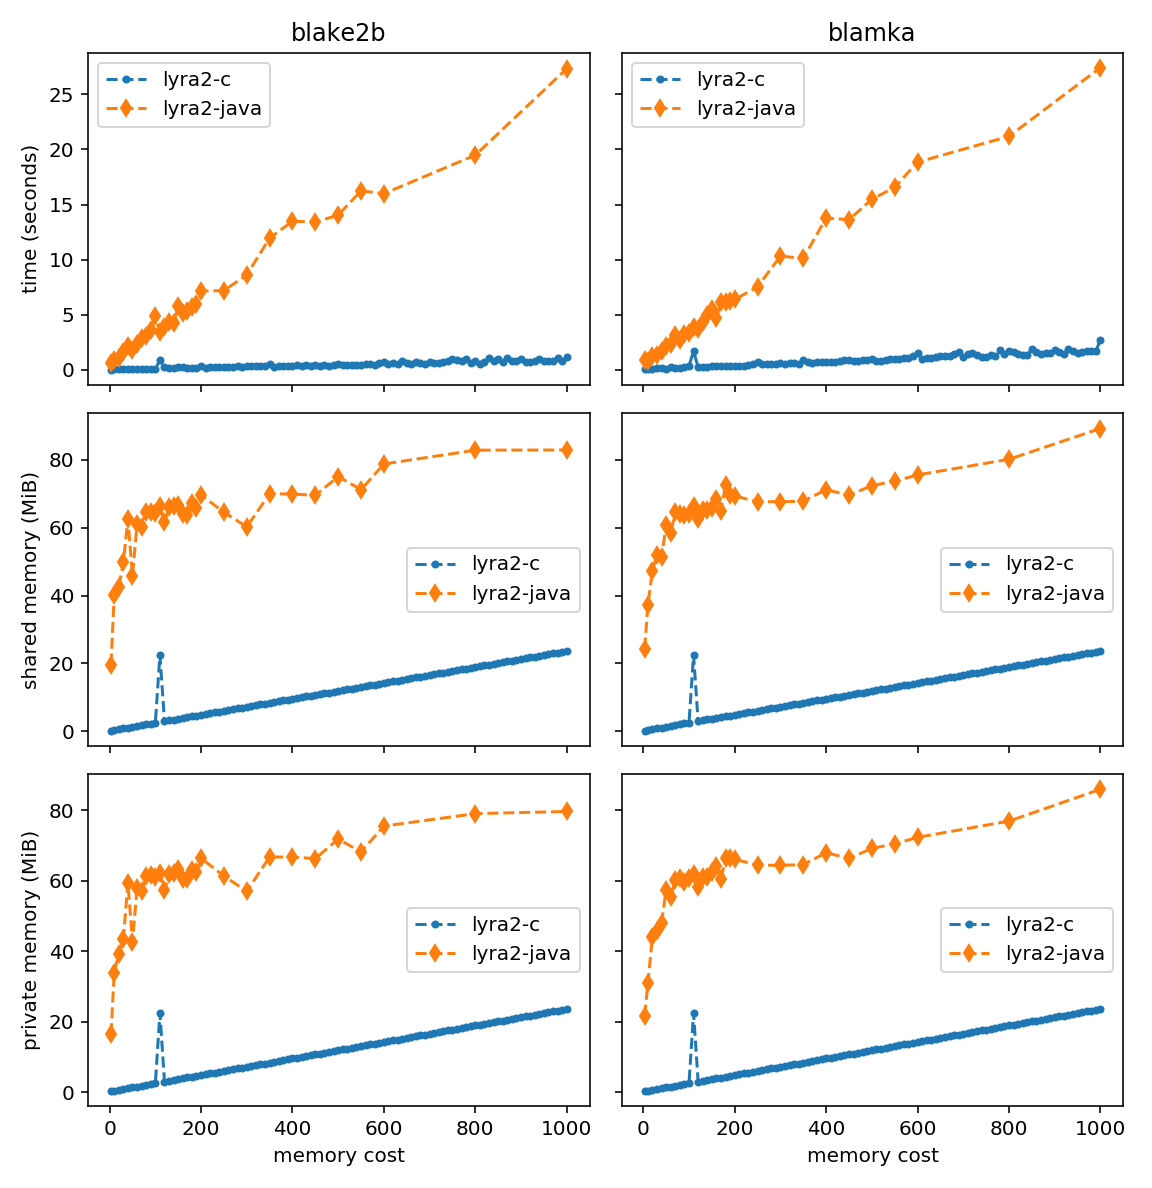
\includegraphics[width=\linewidth,keepaspectratio]{figures/mcost_256}
    \caption{\texttt{lyra2-c} compared to \texttt{lyra2-java}: 256 columns, fixed time cost of 10. Blake2b sponge on the left, BlaMka sponge on the right.}
    \label{figure:mcost_256}
\end{figure}

\begin{figure}[H]
    \centering
    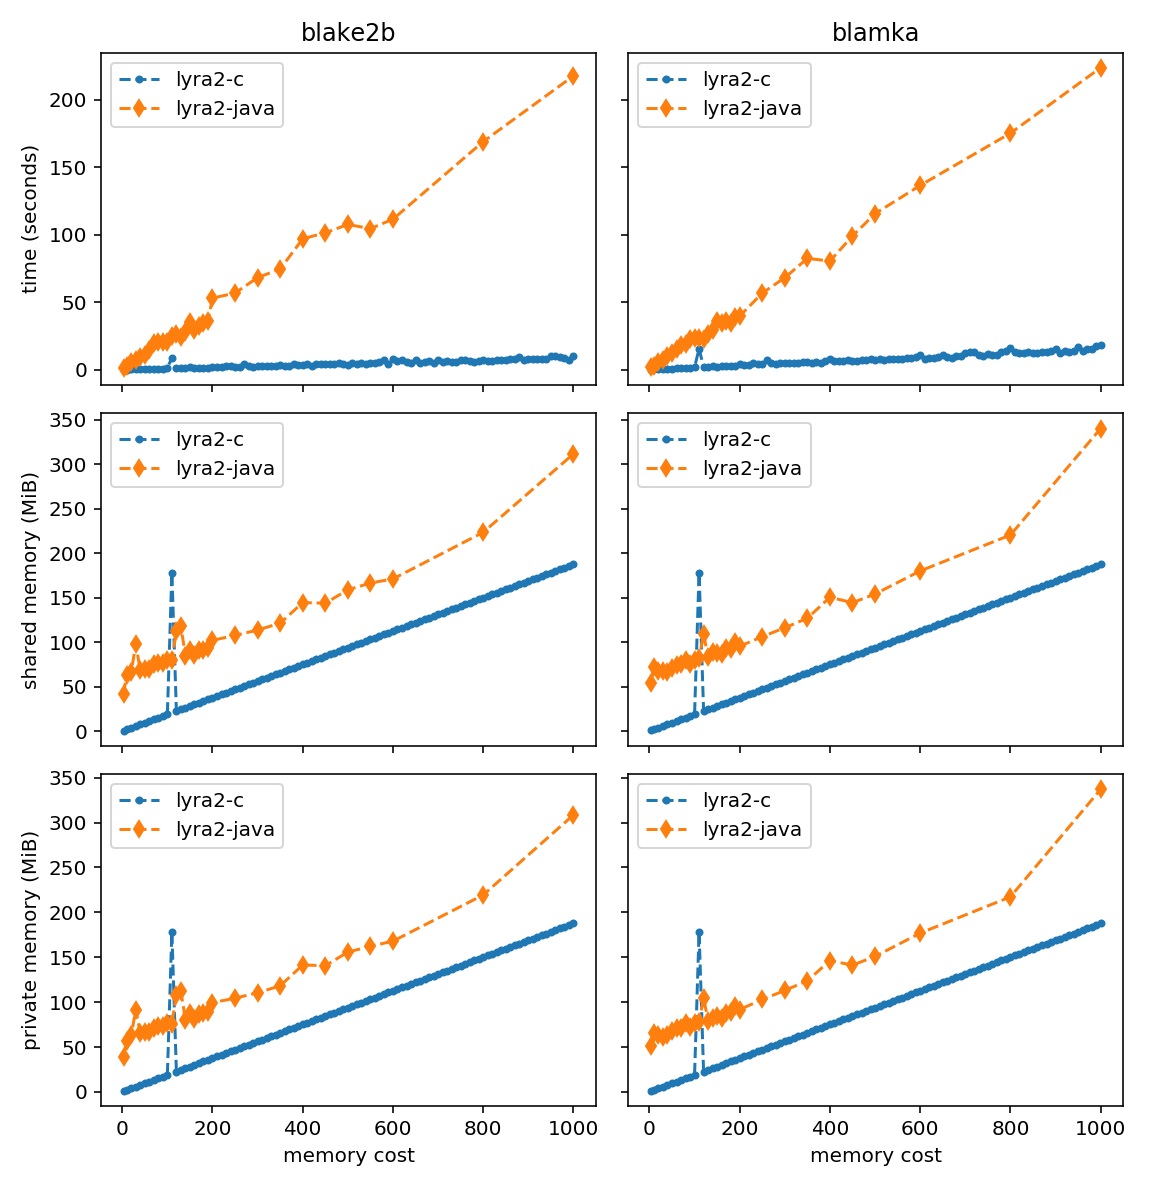
\includegraphics[width=\linewidth,keepaspectratio]{figures/mcost_2048}
    \caption{\texttt{lyra2-c} compared to \texttt{lyra2-java}: 2048 columns, fixed time cost of 10. Blake2b sponge on the left, BlaMka sponge on the right.}
    \label{figure:mcost_2048}
\end{figure}

\subsection{Fixed Memory Cost}
\label{sec:fixed-memory-cost}

There are two figures that show how running time and consumed memory depend on time cost when memory cost is fixed. Figure \ref{figure:tcost_256} shows a 256-column and figure \ref{figure:tcost_2048} shows a 2048-column configuration of Lyra2. Both these figures show that the original C implementation works faster and consumes less memory than its Java counterpart. The running time changes roughly linearly as the time cost parameter is changed which is consistent with the fact that time cost corresponds to the number of iterations done by Lyra2. Memory consumption stays roughly the same which is also consistent with the fact that the largest memory consumer is the in-memory matrix. This matrix has the same size for all of the configurations. Admittedly, there are some deviations in memory consumption of the Java implementation. The second set of figures \ref{figure:tcost_2048} even has a slight downward trend. The possible reasons for that include: the built-in garbage collector and the fact that the measurements run for several days, resulting in potentially different system loads.

\begin{figure}[H]
    \centering
    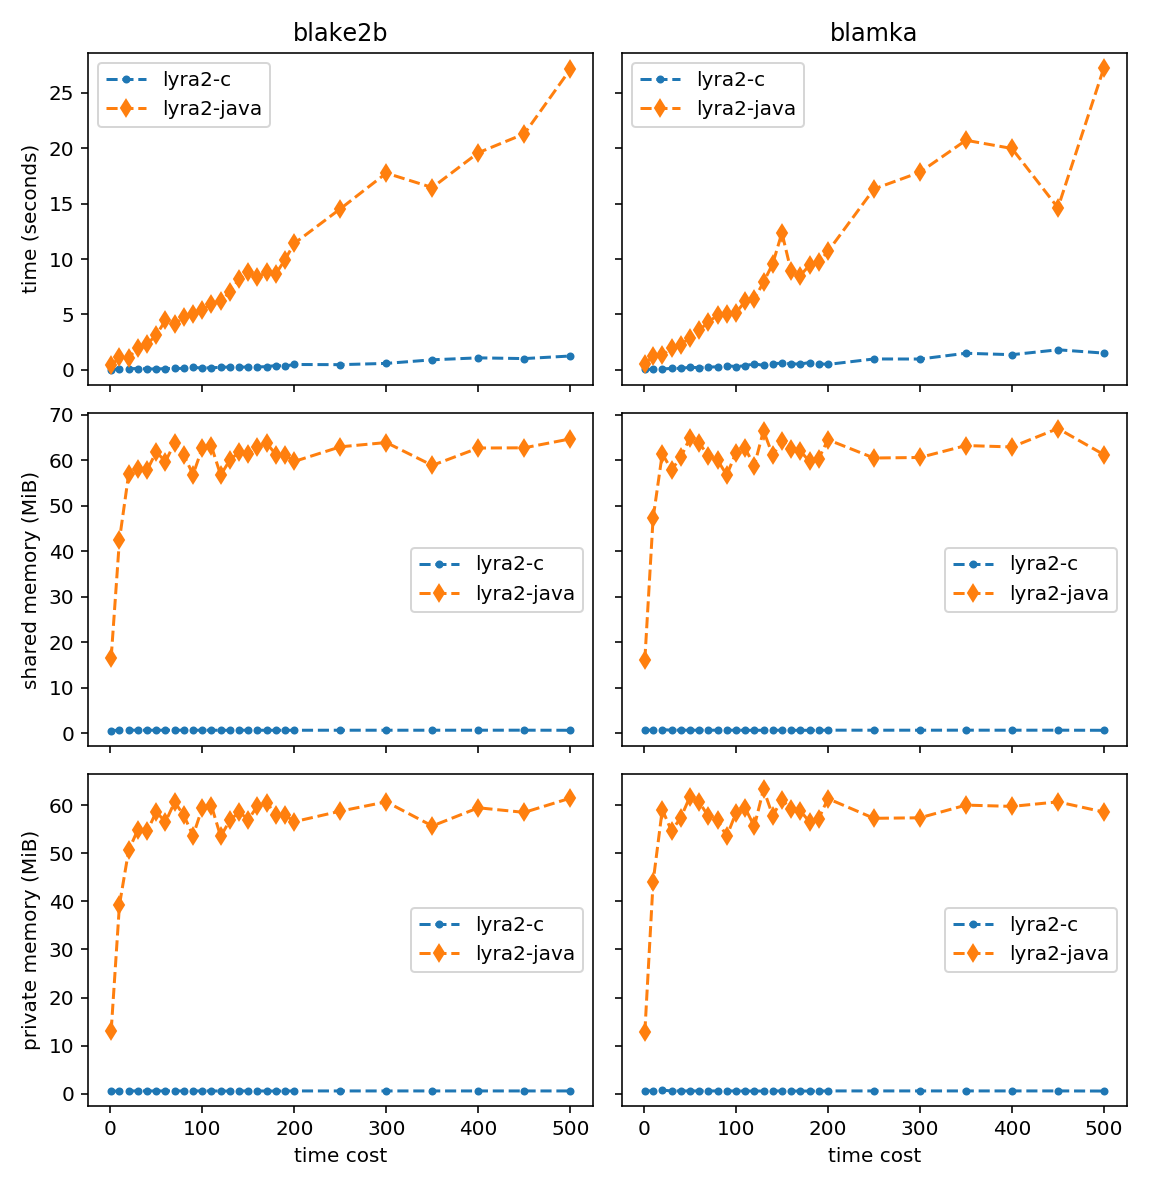
\includegraphics[width=\linewidth,keepaspectratio]{figures/tcost_256}
    \caption{\texttt{lyra2-c} compared to \texttt{lyra2-java}: 256 columns, fixed memory cost of 20. Blake2b sponge on the left, BlaMka sponge on the right.}
    \label{figure:tcost_256}
\end{figure}

\begin{figure}[H]
    \centering
    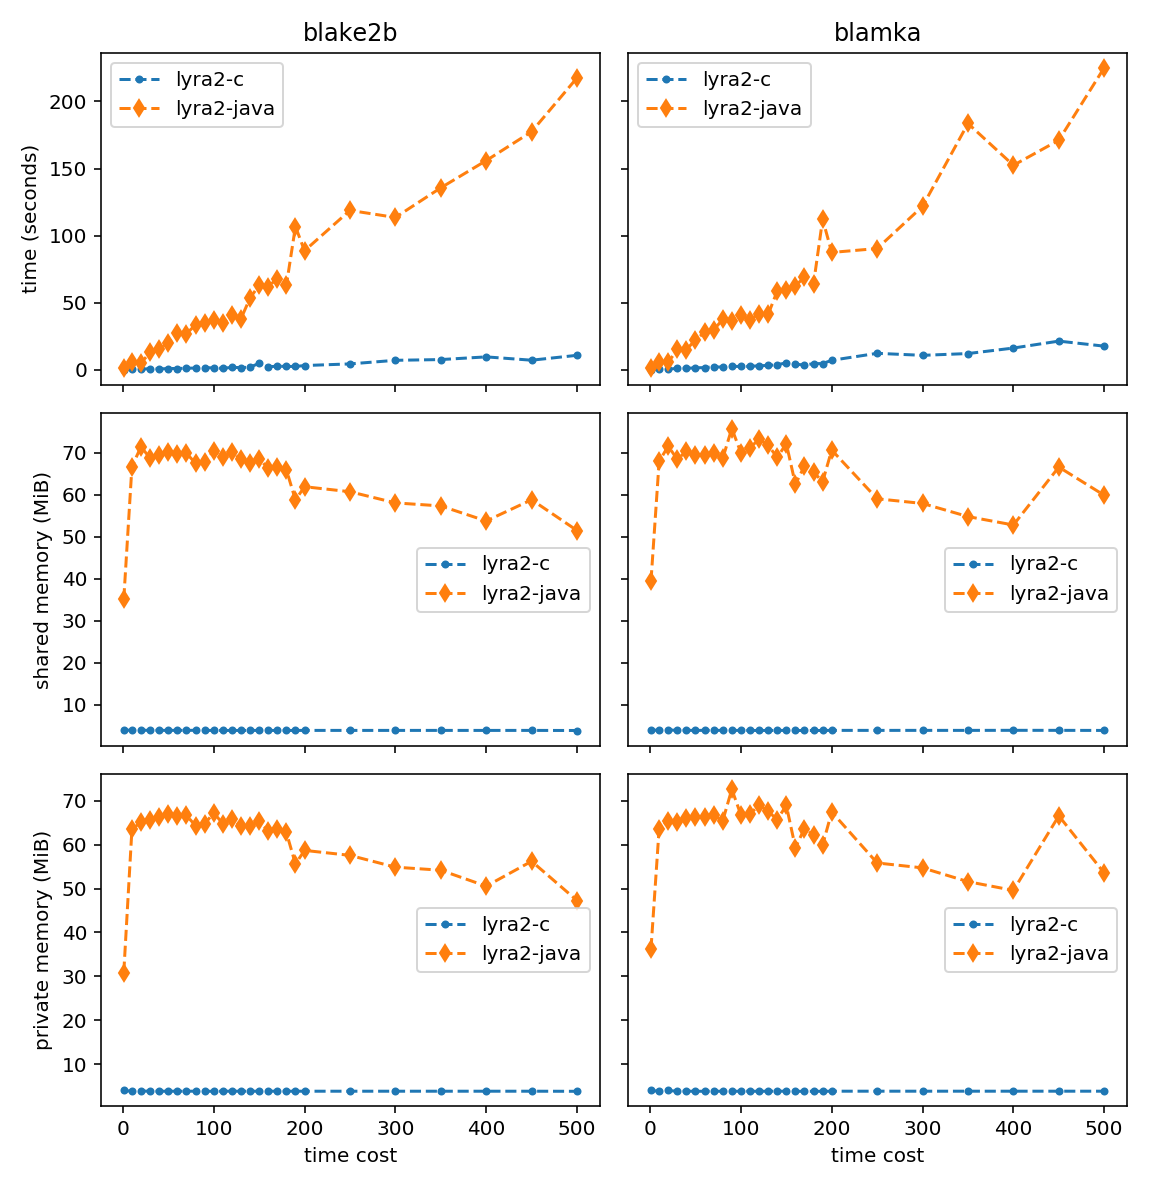
\includegraphics[width=\linewidth,keepaspectratio]{figures/tcost_2048}
    \caption{\texttt{lyra2-c} compared to \texttt{lyra2-java}: 2048 columns, fixed memory cost of 20. Blake2b sponge on the left, BlaMka sponge on the right.}
    \label{figure:tcost_2048}
\end{figure}

\subsection{Variable Time and Memory Costs}
\label{sec:no-fixed-costs}

There are four figures that show running time and memory consumption of Lyra2 when both time and memory costs change. Figures \ref{figure:tcost_mcost_blake2b_256} and \ref{figure:tcost_mcost_blake2b_2048} correspond to a 256- and 2048-column configurations of Lyra2 that both use the Blake2b sponge. Figures \ref{figure:tcost_mcost_blamka_256} and \ref{figure:tcost_mcost_blamka_2048} are the 256- and 2048-column configurations of Lyra2 with the BlaMka sponge. All of these four figures share the same properties. First of all, the reference implementation is faster and consumes less memory than its Java counterpart. Secondly, the running time as well as required space depend roughly linearly on the time and memory cost parameters. However, together they create a quadratic time growth during the \emph{Wandering phase}. This still allows for predictable and fine-tuned control of the time and memory resources required by the algorithm.

\begin{figure}[p]
    \centering
    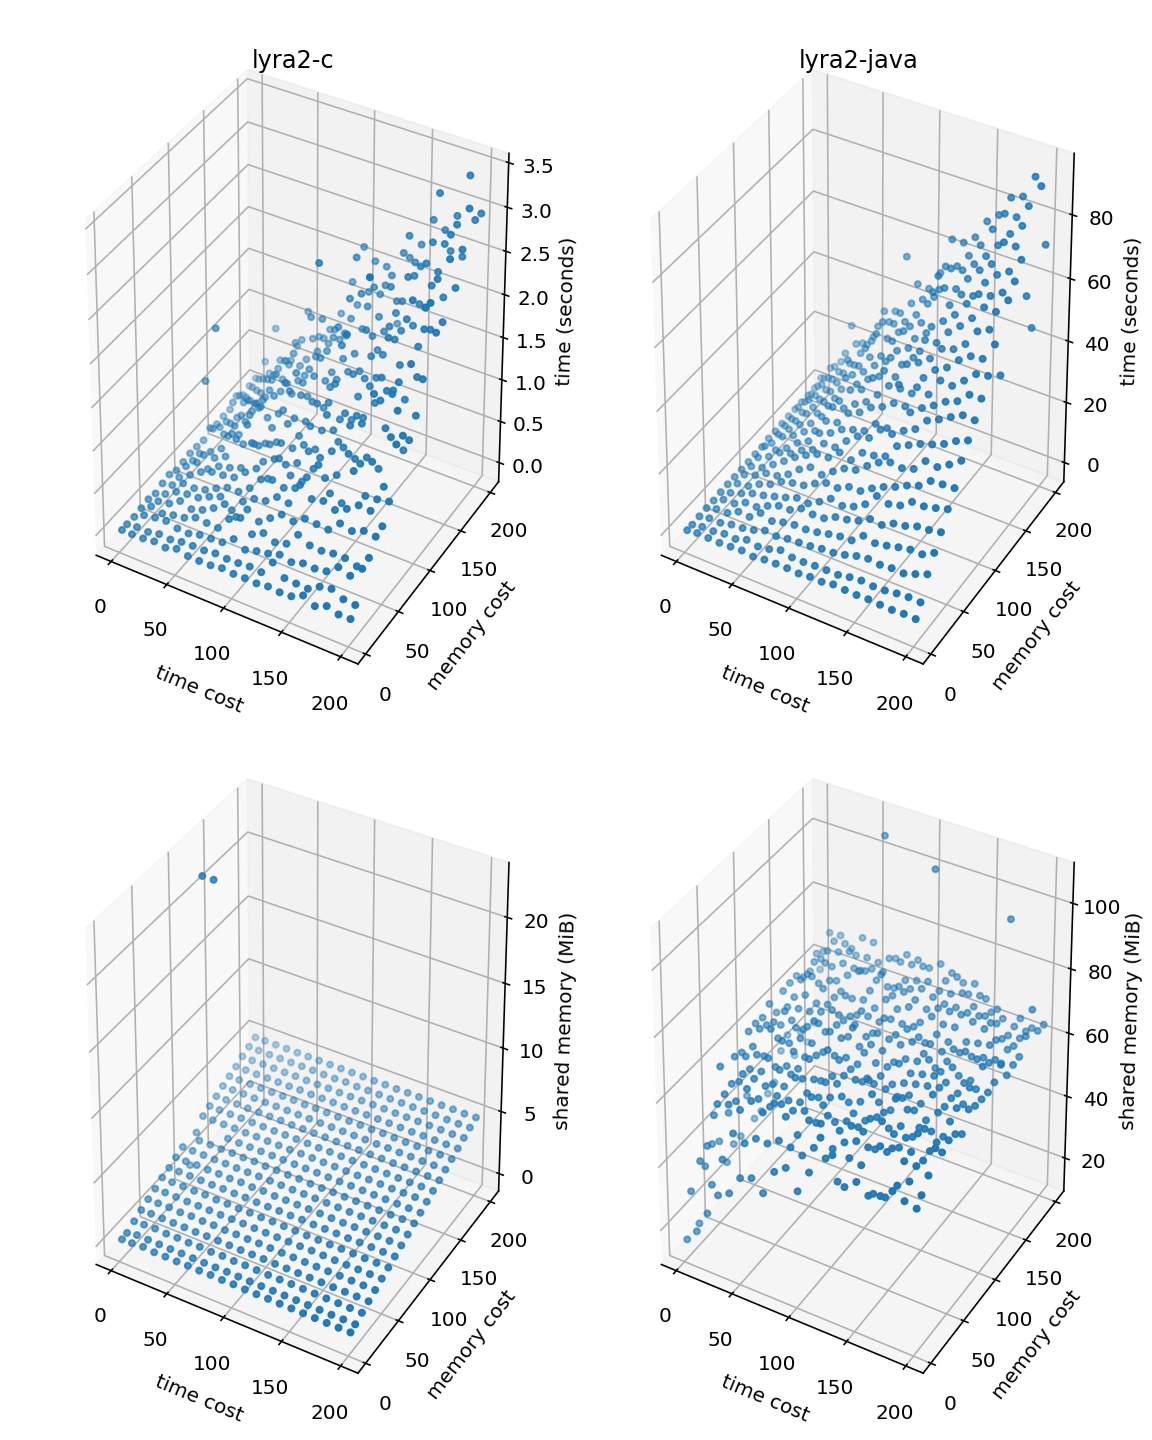
\includegraphics[width=\linewidth,keepaspectratio]{figures/tcost_mcost_blake2b_256}
    \caption{\texttt{lyra2-c} compared to \texttt{lyra2-java}: Blake2b sponge, 256 columns.}
    \label{figure:tcost_mcost_blake2b_256}
\end{figure}

\begin{figure}[p]
    \centering
    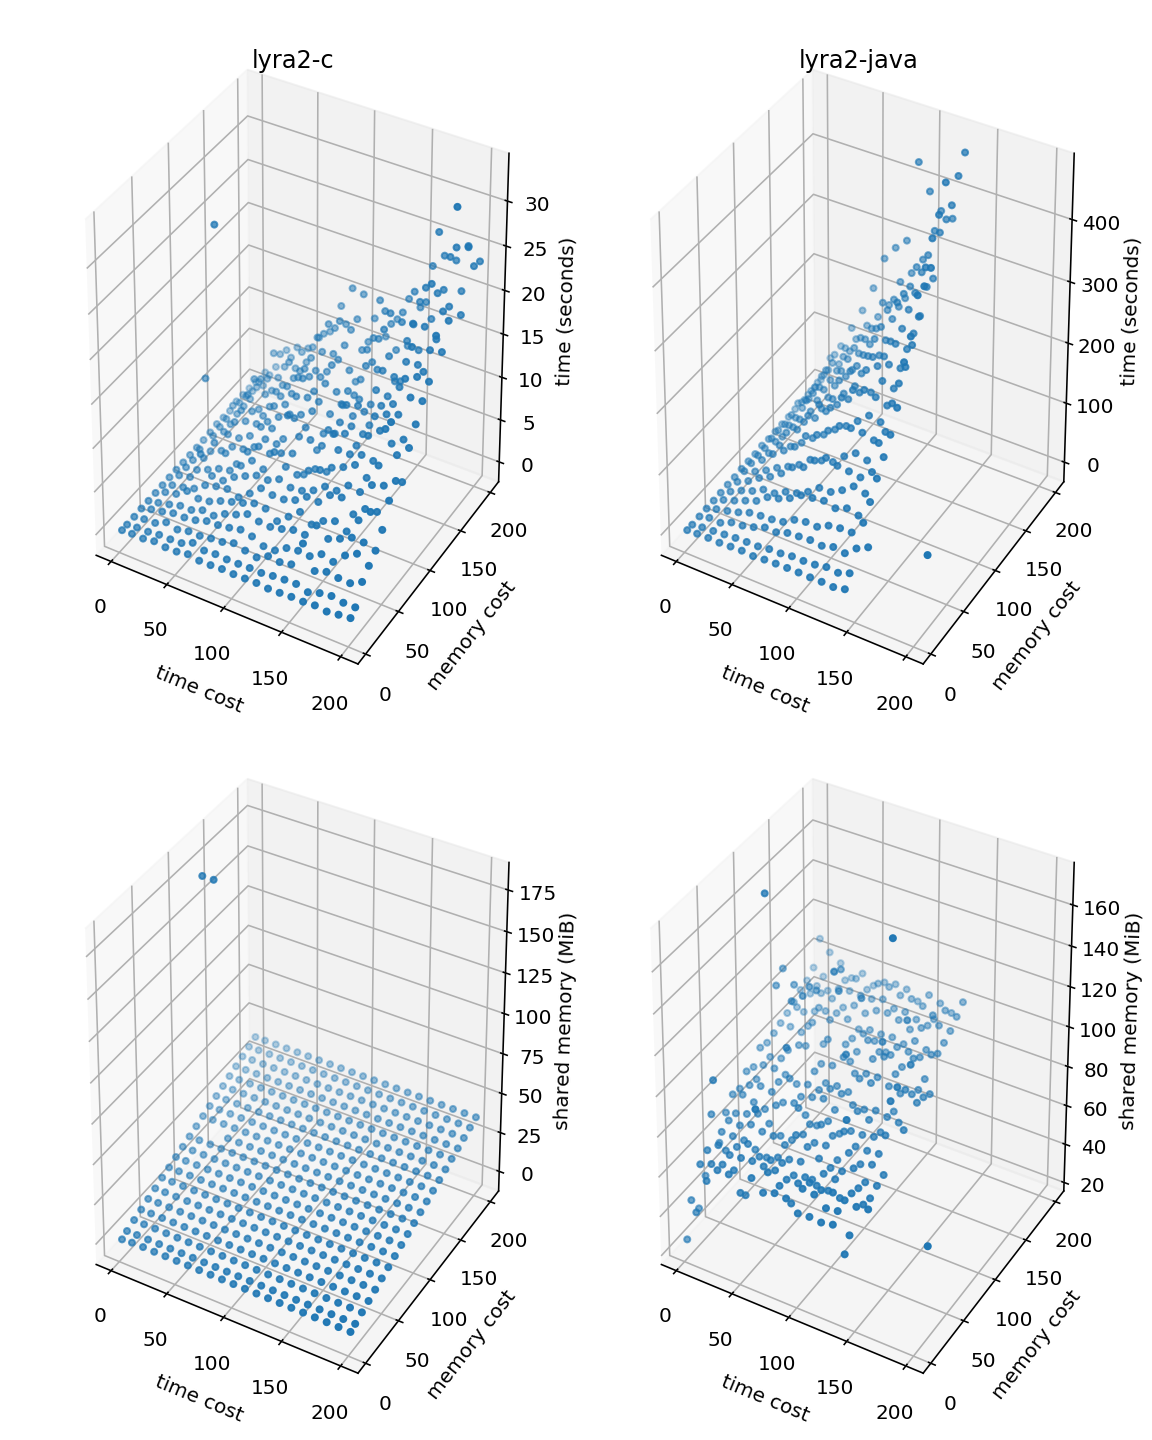
\includegraphics[width=\linewidth,keepaspectratio]{figures/tcost_mcost_blake2b_2048}
    \caption{\texttt{lyra2-c} compared to \texttt{lyra2-java}: Blake2b sponge, 2048 columns.}
    \label{figure:tcost_mcost_blake2b_2048}
\end{figure}

\begin{figure}[p]
    \centering
    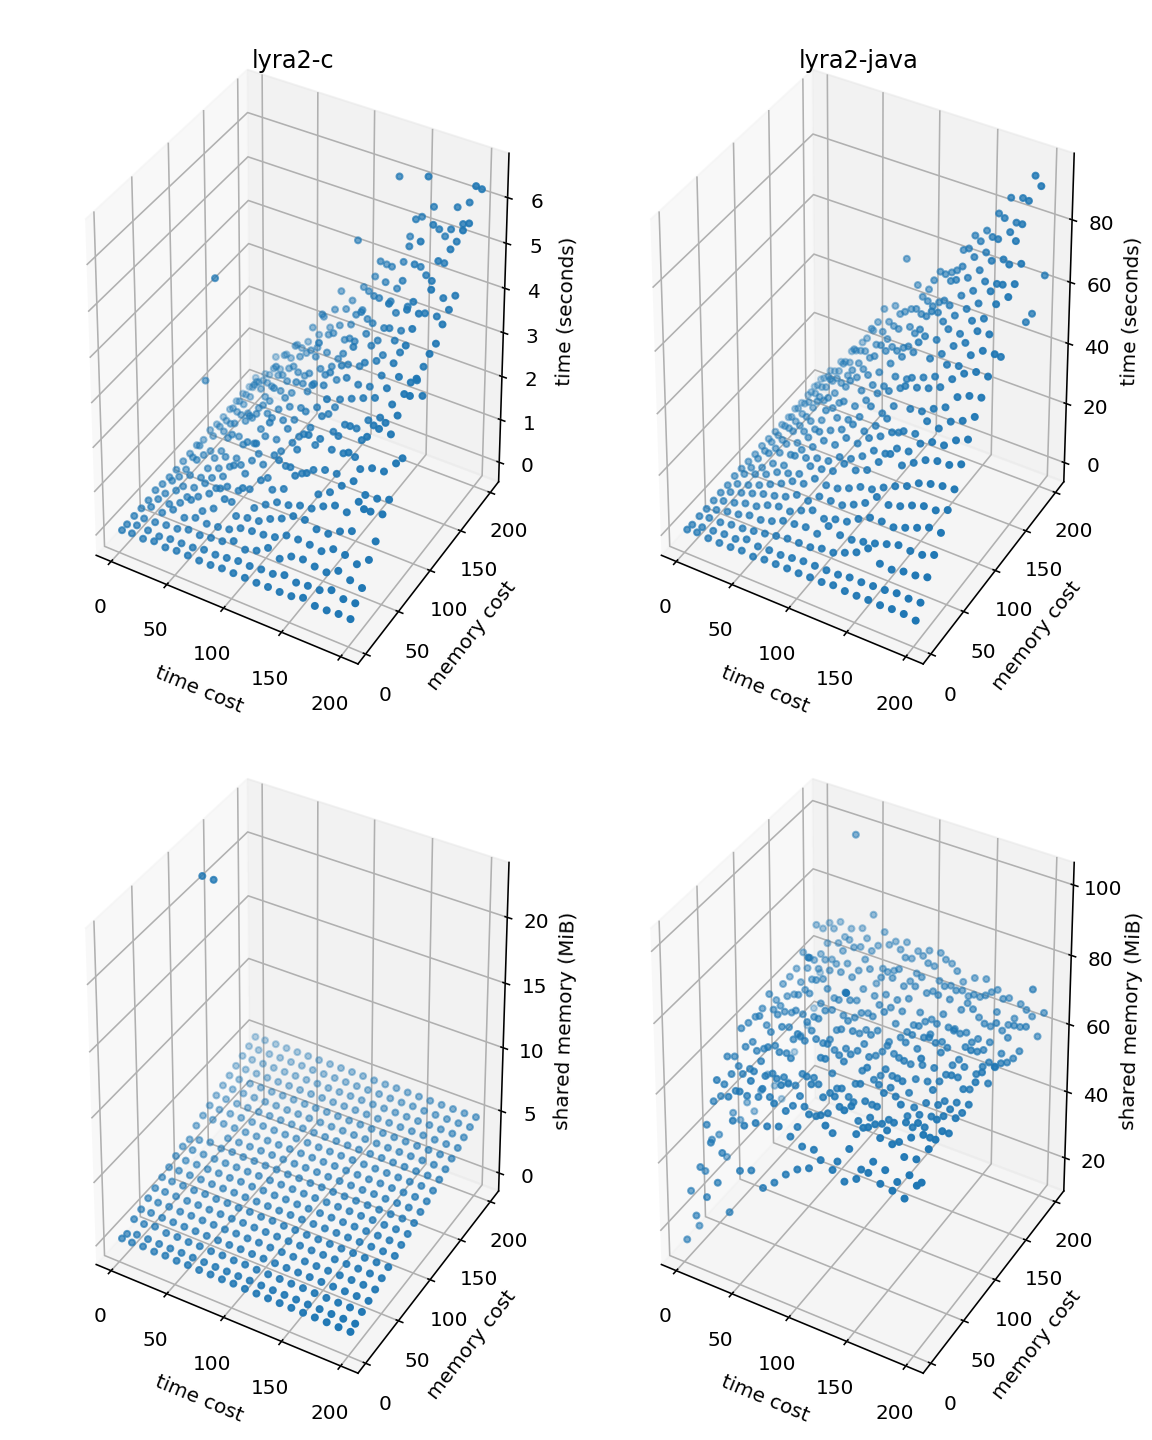
\includegraphics[width=\linewidth,keepaspectratio]{figures/tcost_mcost_blamka_256}
    \caption{\texttt{lyra2-c} compared to \texttt{lyra2-java}: BlaMka sponge, 256 columns. }
    \label{figure:tcost_mcost_blamka_256}
\end{figure}

\begin{figure}[p]
    \centering
    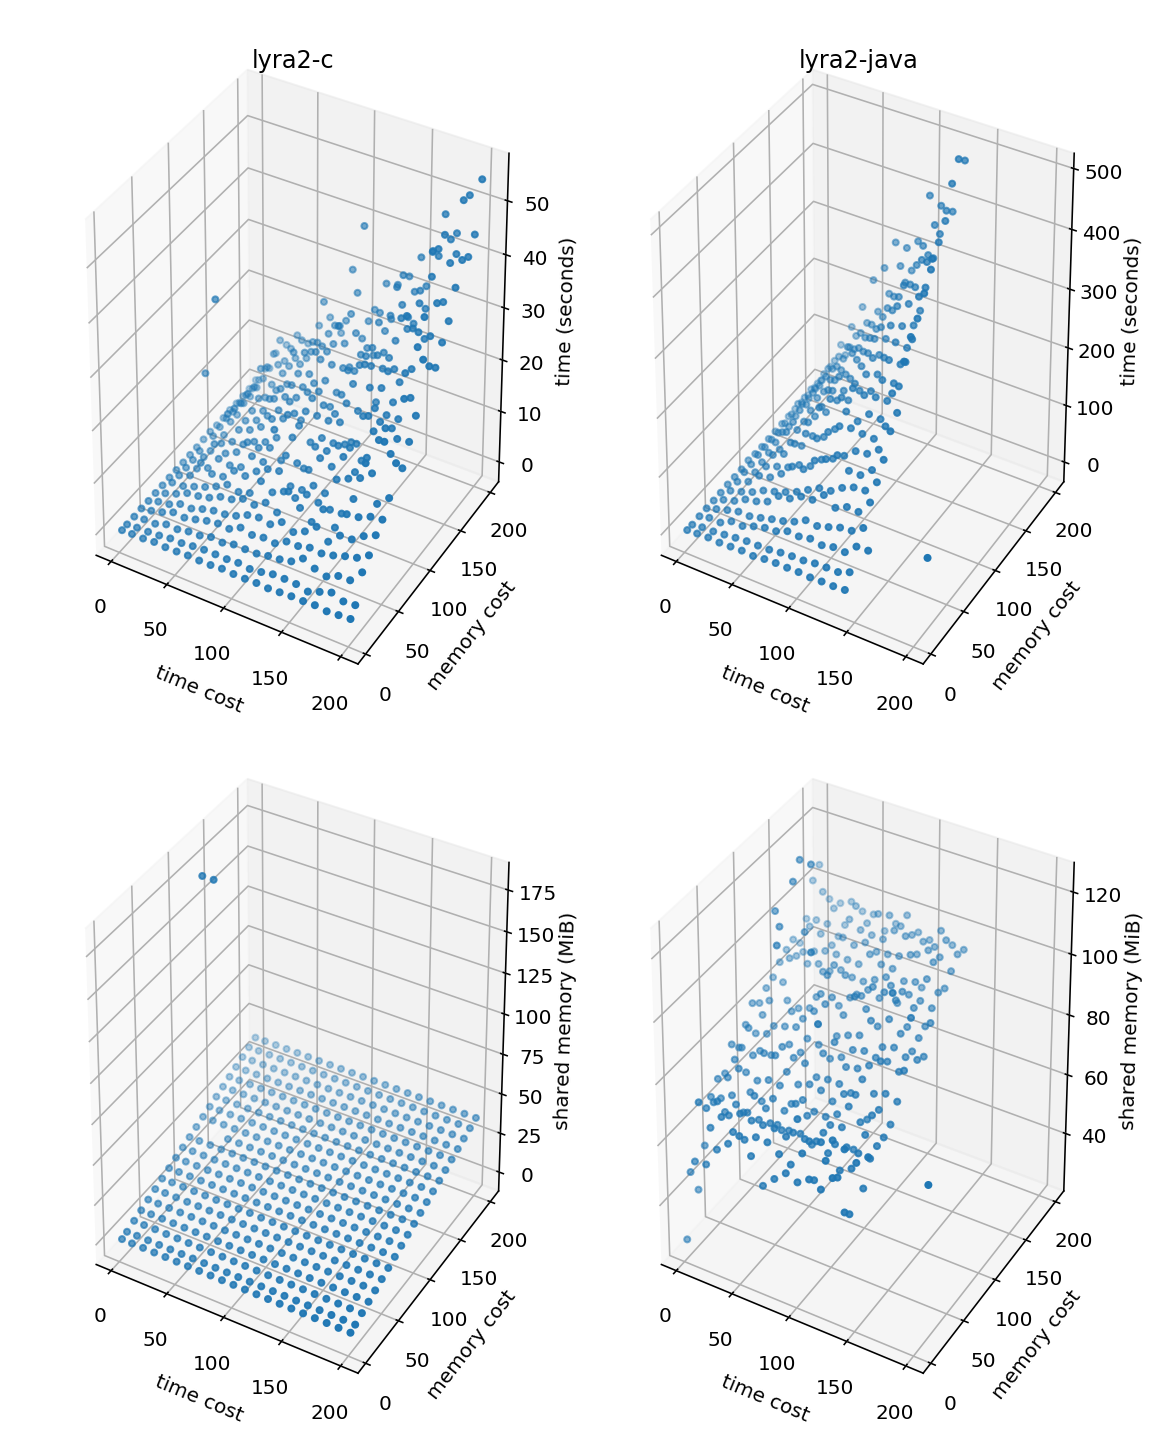
\includegraphics[width=\linewidth,keepaspectratio]{figures/tcost_mcost_blamka_2048}
    \caption{\texttt{lyra2-c} compared to \texttt{lyra2-java}: BlaMka sponge, 2048 columns.}
    \label{figure:tcost_mcost_blamka_2048}
\end{figure}

\clearpage
\subsection{Comparison Conclusion}
\label{sec:comparison-conclusion}

The Java implementation was outperformed by the reference C implementation. This could in part be attributed to language ecosystems or programming skills but it also cannot be denied that the ported version takes a lot of extra steps in order to ensure algorithm-level compatibility. These include the extra rotations requried to simulate little-endian behaviour, as well as simulating pointer arithmetic or unsigned arithmetic for large 64-bit integers.

\section{Android Application}
\label{sec:mobile-application}

Part of the porting effort is a small proof of concept mobile application. This application demonstrates that using a native Java library in an Android project is convenient.

One of the first steps is to determine the minimum versions of Android devices and API levels necessary. Since lyra2-java makes use of unsigned 64-bit number arithmetic, Java 1.8 support is required. This translates into the minimum Android versions of 7.0 and the API level of 24 \footnote{https://developer.android.com/guide/platform/j8-jack.html (visited on 10/23/2017)}.

The most common development environment for Android applications is the Android Studio. Support for Java 1.8 features has not yet landed into the release version of this IDE. So, in order to be able to develop a mobile application with Lyra2, a development version \texttt{3.0} needs to be installed. If you encounter a (similar) traceback as shown in figure \ref{fig:traceback}, there are several possible workarounds available online. The most effective one is to instruct Android Studio to use system libraries:

\begin{minted}{shell}
ANDROID_EMULATOR_USE_SYSTEM_LIBS=1 ./studio.sh
  \end{minted}

\begin{figure}
\begin{minted}{shell}
    Emulator: libGL error: unable to load driver: i965_dri.so
    Emulator: libGL error: driver pointer missing
    Emulator: libGL error: failed to load driver: i965
    Emulator: libGL error: unable to load driver: i965_dri.so
    Emulator: libGL error: driver pointer missing
    Emulator: libGL error: failed to load driver: i965
    Emulator: libGL error: unable to load driver: swrast_dri.so
    Emulator: libGL error: failed to load driver: swrast
    Emulator: X Error of failed request:  BadValue (integer parameter out of range for operation)
    Emulator: Major opcode of failed request:  155 (GLX)
    Emulator: Minor opcode of failed request:  24 (X_GLXCreateNewContext)
    Emulator: Value in failed request:  0x0
    Emulator: Serial number of failed request:  42
    Emulator: Current serial number in output stream:  43
    Emulator: Process finished with exit code 1
\end{minted}
\caption{Android Studio emulator: an obscure error traceback connected to \texttt{libGL}.}
\label{fig:traceback}
\end{figure}

Once these preliminary steps are performed, the development of the application becomes straightforward. Android Studio is based on IntelliJ Studio and therefore picks up lyra2-java from the Maven Central repository in a matter of a couple clicks.

As a result, a simple Android application was developed and is available on GitHub \cite{github:2017:lyra2-mobile}. It consists of a main screen and a results screen. The main screen allows the user to choose the particular configuration of Lyra2. By default, the Blake2b sponge with the time and memory cost of 100 will be used. The password and salt fields are set to the default values of "password" and "salt" respectively, the number of columns is 256 with each column being 12 blocks wide. The permutation inside the sponge makes a total 12 rounds of computations. All of the parameters above can be adjusted.

Figure \ref{fig:lyra2-mobile-demo} demonstrates the hash value after running with default parameters as well as the hash value when using BlaMka instead of Blake2b. The hash values match those from the manual testing section \ref{sec:manual-testing}. In each case the computation lasted for approximately 60 seconds which is consistent with the desktop version times. However, it should be noted that the application was tested in an emulator and not on an actual device.

\begin{figure}[H]
\centering
\begin{subfigure}{.5\textwidth}
  \centering
  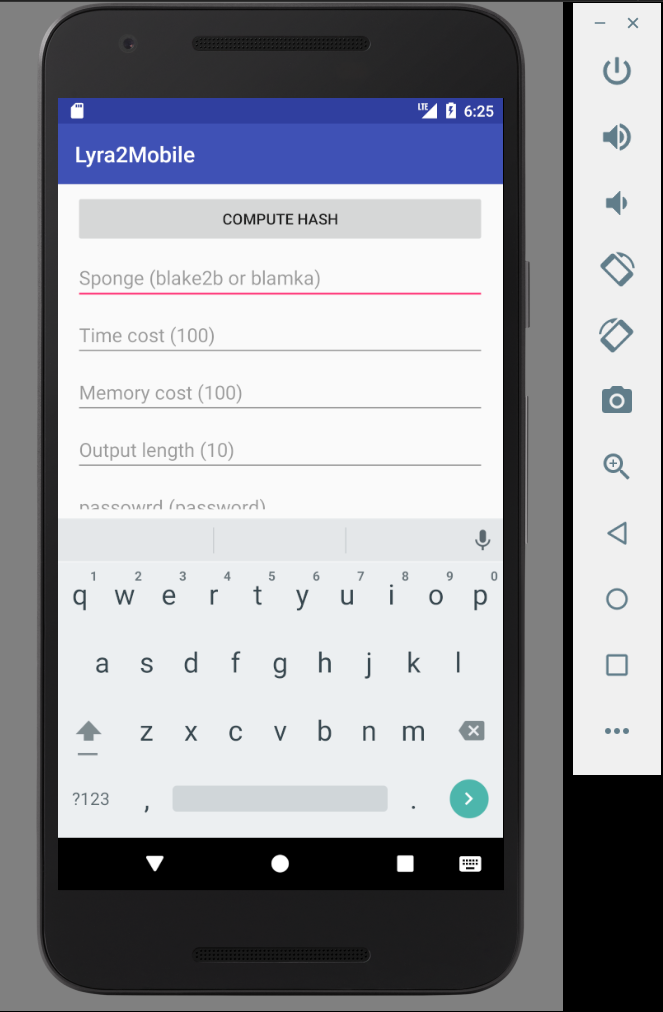
\includegraphics[width=.8\linewidth]{figures/lyra2-mobile-main-clean}
  \caption{Main screen (Blake2b sponge, default)}
  \label{fig:lyra2-mobile-main}
\end{subfigure}%
\begin{subfigure}{.5\textwidth}
  \centering
  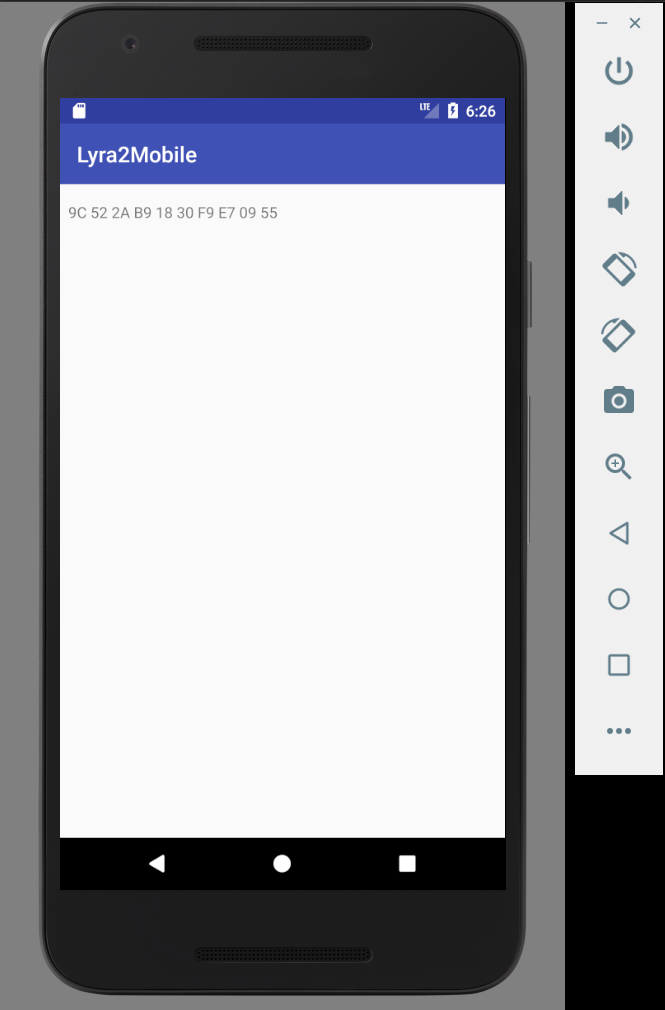
\includegraphics[width=.8\linewidth]{figures/lyra2-mobile-result-clean}
  \caption{Resulting hash (Blake2b sponge, default)}
  \label{fig:lyra2-mobile-result}
\end{subfigure}
\begin{subfigure}{.5\textwidth}
  \centering
  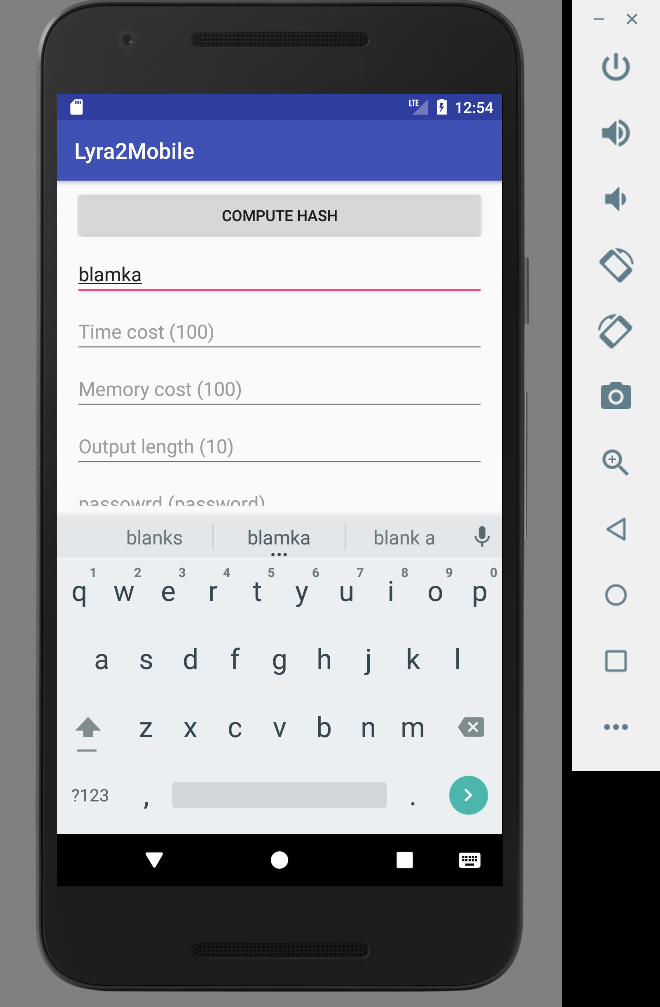
\includegraphics[width=.8\linewidth]{figures/lyra2-mobile-main-blamka-clean}
  \caption{Main screen (BlaMka sponge)}
  \label{fig:lyra2-mobile-main}
\end{subfigure}%
\begin{subfigure}{.5\textwidth}
  \centering
  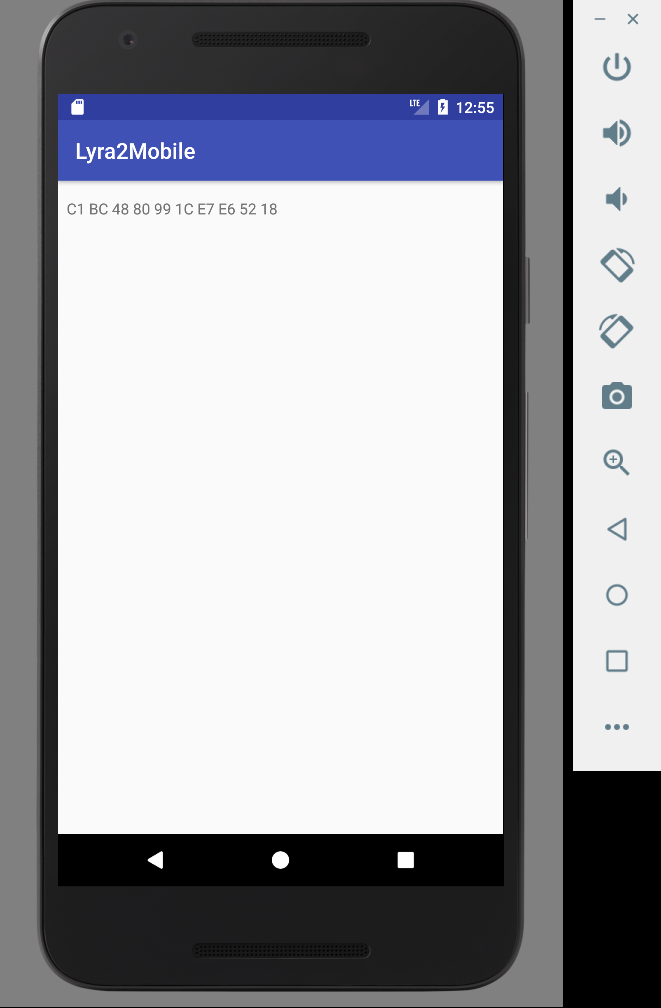
\includegraphics[width=.8\linewidth]{figures/lyra2-mobile-result-blamka-clean}
  \caption{Resulting hash (BlaMka sponge)}
  \label{fig:lyra2-mobile-result}
\end{subfigure}
\caption{Android application running Lyra2. Each of the two configurations runs for \(\approx 60\) seconds. Parameter values on the left, resulting hash in hexadecimal on the right.}
\label{fig:lyra2-mobile-demo}
\end{figure}

\makeatletter\ifthesis@masterthesis
%%%%%%%%%%%%%%%%%%%%%%%%%%%%%%%%%%%%%%%%%%%%%%%%%%%%%%%%%%%%%%%%%%%%%%%%
\chapter{Diskussion}
\label{sec:discussion}
%%%%%%%%%%%%%%%%%%%%%%%%%%%%%%%%%%%%%%%%%%%%%%%%%%%%%%%%%%%%%%%%%%%%%%%%

Den akademischen Wert der Arbeit hervorheben, Vergleich mit verwandten Arbeiten: In welchem Verhältnis stehen die Ergebnisse der Diplomarbeit zu den Ergebnissen anderer Studien? Wo gibt es Unterschiede, wo Gemeinsamkeiten? Warum?

Diskussion offener Punkte, Darstellen der Stärken und Schwächen der vorliegenden Ergebnisse.
\fi\makeatother
%%%%%%%%%%%%%%%%%%%%%%%%%%%%%%%%%%%%%%%%%%%%%%%%%%%%%%%%%%%%%%%%%%%%%%%%
\chapter{Zusammenfassung und Ausblick}
\label{sec:conclusion}
%%%%%%%%%%%%%%%%%%%%%%%%%%%%%%%%%%%%%%%%%%%%%%%%%%%%%%%%%%%%%%%%%%%%%%%%

\makeatletter\ifthesis@masterthesis
Die Zusammenfassung ist nach der Kurzfassung der am häufigsten gelesene Teil, da viele Leser aus Zeitknappheit Arbeiten im Schnellverfahren konsumieren und rasch zur Zusammenfassung blättern. Hier hat man die Chance, dem Leser noch einmal die zentralen Ideen und Ergebnisse der Diplomarbeit zu vermitteln.

Im Gegensatz zur Kurzfassung sind die Leser mit der Problemstellung und der Terminologie bereits vertraut. In der Länge hat man deutlich mehr Spielraum als bei der Kurzfassung, die Zusammenfassung sollte inklusive Ausblick 2 bis max. 10 Seiten umfassen. Hier sollten kompakt die Antworten auf die in der Zielsetzung aufgeworfenen Fragen (Hypothesen) gegeben werden.

Neben einer Zusammenfassung der wichtigsten Ergebnisse sollte auch ein Ausblick gegeben werden: Aufzeigen des Bedarfs an zukünftiger Forschung, potentielle Anwendungsmöglichkeiten der vorgestellten Lösung etc.

In Summe sollte die Zusammenfassung dem Leser die wissenschaftliche und, wenn vorhanden, praktische Relevanz der Arbeit klar und verständlich darlegen.
\fi\makeatother

% insert bibliography and such stuff
\BackMatter

\cleardoublepage
\appendix

\chapter{Android Studio Preview}
\label{chapter:problem?}

At the moment using Lyra2 in an Android application requires a beta (i.e. preview) version of Android Studio. The instructions on the official webpage \footnote{https://developer.android.com/studio/preview/index.html} warn the developer about the need to update plugins. However, this is not the only problem which you may face when running the preview version.

If you require an emulator to test the application, you may be treated with the following  error traceback presented in \ref{fig:traceback}. Different kinds of advice is supposed to help with the problem: preloading the \texttt{libstdc++.so.6} library ahead of time, adding the user who runs Android Studio to the \texttt{video} group, etc. On my machine (a ThinkPad E570 notebook with a dedicated GTX 950M graphics card running ArchLinux), the solution that worked was to instruct Android Studio to rely on system libraries. This can be achieved by setting an environment variable:

\begin{minted}{shell}
ANDROID_EMULATOR_USE_SYSTEM_LIBS=1 ./studio.sh
  \end{minted}

\begin{figure}
\begin{minted}[fontsize=\tiny]{shell}
    Emulator: libGL error: unable to load driver: i965_dri.so
    Emulator: libGL error: driver pointer missing
    Emulator: libGL error: failed to load driver: i965
    Emulator: libGL error: unable to load driver: i965_dri.so
    Emulator: libGL error: driver pointer missing
    Emulator: libGL error: failed to load driver: i965
    Emulator: libGL error: unable to load driver: swrast_dri.so
    Emulator: libGL error: failed to load driver: swrast
    Emulator: X Error of failed request:  BadValue (integer parameter out of range for operation)
    Emulator: Major opcode of failed request:  155 (GLX)
    Emulator: Minor opcode of failed request:  24 (X_GLXCreateNewContext)
    Emulator: Value in failed request:  0x0
    Emulator: Serial number of failed request:  42
    Emulator: Current serial number in output stream:  43
    Emulator: Process finished with exit code 1
\end{minted}
\caption{An obscure error traceback connected to \texttt{libGL}.}
\label{fig:traceback}
\end{figure}


\end{document}
